\part{Behavioral Disease Model}

\chapter{Epidemic and Behavioral model alone: a presentation}



To develop a multi-layer network combining an epidemiological layer with a behavioral one, we first study the dynamics of each layer separately, as presented here. 

In this section, we describe the developed SIRS epidemiological model, followed by the Careless, Compliant, Against behavioral model. A sensitivity analysis is also conducted. Understanding the underlying dynamics of each graph is crucial for better comprehending the dynamics emerging from the multi-layer structure.


\section{SIRS model}
\label{sec:SIRS}

$\beta$ is the transmission rate parameter for person-to-person
contact, $\gamma$ is the recovery rate, $\delta$ is the rate at which
immunity recedes following recovery, and $R(t)$ is the recovered
fraction of the population

To describe the epidemic evolution a  SIRS model is implemented. It is an extension of the most famous SIR. Its main addition is the possibility for individuals to become again susceptible after a certain period of time beyond the end of the infection. The choice of a SIR-like model is done because they are well-known as capable to describe disease like the COVID-19 CITA. From an epidemiological point of view, an "Exposed" compartment will be very suitable, to describe better the evolution of the disease. In fact, in this class of infections, after the contact with an infectious there is a certain period of incubation before the development of symptoms and contagiousness. Nevertheless this compartment was not insert in the model, because it was demonstred CITA, that also a more simple SIR can be able to model correctly the disease. In this case for realise a better fit of the real data a delay in the time scale of the system can be added in the model. This delay can be considered as an extra time to ... CITA E VEDI ARTICOLO.

The possibility of become again susceptibles is added in the model, because it is considered an interesting feature in the study of a long range time scenario. 
Considering the effect of people behaviour on the evolution of a disease, it is hypothesized that two keys moment of this influence can be the initial stages and after the first peak of epidimic. 
All'inizio il sirs si comporterà come un modello sir normal, perchè non ci saranno abbbastanza tempo trascorso perchè le persone possano reinfettarsi. Però dopo le persone posso no reinfettarsi e la loro opinione e comportamento diventerà importante. da spiegare meglio

\section{Behavioural model}
The behavioural network alone is composed of three compartments.
These are Compliant, $Co$, Careless $Ca$, Against $Ag$. 
The differential equations describing the model evolution are \ref{eq:behavioural_eq}: 
\begin{equation}
	\begin{cases}
		\dot{Ca} = -k_1 Ca Co - k_2 Ca Ag + \lambda_1 Co + \lambda_2 Ag \\
		\dot{Co} = k_1 Ca Co -  \lambda_1 Co \\
		\dot{Ag} = k_2 Ca Ag -  \lambda_2 Ag\\
	\end{cases}
	\label{eq:behavioural_eq}
\end{equation}
As initial condition the hypothesis is that at the start time of the simulation most of the population is in the Careless compartment. It is considered that if a new infection developed, it is not well known and so population have little information about it. The Careless compartment is composed by people that do not know about the risk associated with becoming infected, or that have not sufficient fear of the infection to modify their normal behaviour. 
As an example of this possible initial configuration it is considered the covid-19 case in Italy. At the early stage of its development, when the disease was spreading in China it was not considered a menace for most of the population in western countries. It is seen as a disease involving a different and far state. So, when the epidemic arrives in Europe and Italy, both the population and the government did not expect it and there is an initial time delay before the countermeasures were activated and before reliable information about the evolution of the disease are available to the population. 
There are then two opposite behavioural standings: Compliant and Against.
In the Compliant set there are population worried about the disease and that want to reduce their possibilities of becoming infected. Conversely, the Against is formed by a group of individuals that have anti-scientific ideas about the disease. Here are summarised phenomena like:
\begin{itemize}
		\item vaccine denialism;
		\item misinformation diffusion;
		\item refusal about existence of the disease;
		\item lack of trust on doctors and government policies.
\end{itemize}

%The idea of having the Against compartment is born, because specially in the early phase of a new disease diffusion, there is a lack of reliable knowledge. This documented CITA event can cause the spread of wrong beliefs in the population. It has also been demonstrated CITA that the effect of false information can eradicate, if associated with fears. The most famous example is the conviction about the possibility that vaccine against rosolioa eccettera can generate autism in child. Even if the original publication describing this effect has been scientifically disproved, this idea is still today the most popular and had caused a reduction in the percentage of vaccine population, the so-called “free rider problem”. CITA
For the study of model evolution different coefficient values has been considered.  The rates studied in the models have the following meaning:
\begin{itemize}
	\item $k_1$ influence rate between Ca and Co;
	\item $k_2$ influence rate between Ca and Ag;
	\item $\lambda_1$ rate of leave compliant behaviour due to fatigue;
	\item $\lambda_2$ rate of leave against behaviour due to fatigue.
\end{itemize}

The behaviour of the model is influenced by the value of each of this parameter. For example if the compliant have strong influence, the equilibrium of the model will be composed by most of the population with Compliant behaviour and an Against groups that tend to zero. On contrary, the opposite group composition will be the result. However, if the fatigue due to being Against is less than the one related with being Compliant the final equilibrium can be favourable w.r.t the Against group, even if the rate of $k_1 \ge k_2$.
These effects can be explained looking at the equilibrium for time that goes to infinite. It is found that depends on comparison between the ratios that can be calculated with the formula: 
\begin{equation}
	R_i =\frac{ k_i }{\lambda_i}
	\label{eq:behave_rate}
\end{equation}
This expression is the reproductive ratio of each behaviour. The behaviour with the grater value has a dominant effect on the final stable value reached by the compartments.

\subsubsection{Equilibrium and stability analysis}
There are different final equilibrium value of the system depending on the values of the parameters. In particular, the four coefficients are combined, obtaining two reproduction rates $R_1,R_2$. 
First the nullclines lines are calculated and plotted. To do this, the system can be reduced to two equations assuming the mass conservation and that the following relation holds:
$N=Ca+Co+Ag$
Then the first  two equations are rewritten, rescaling also Ca,Co,Ag with N, the humans population. Using mass conservation condition the Ag term can be substituted in the first equation, resulting in a system of two equations with two unknowns. 
The nullclines lines are calculated and varying the R1 and R2 values the different scenarios are evaluated. 
\[
\begin{cases}
	\dot{Ca} = -k_1 Co Ca - k_2 (N-Co-Ca) Ca + \lambda_1 Co + \lambda_2 (N-Co-Ca)\\
	\dot{Co} = k_1 Co Ca - \lambda_1 Co
\end{cases}
\]
The equations become
\[
\begin{cases}
	\dot{x} = -k_1 y x - k_2 (1-y-x) x + \lambda_1 y + \lambda_2 (1-y-x)\\
	\dot{y} = k_1 y x - \lambda_1 y
\end{cases}
\]
The nullclines lines can be calculated imposing $\dot{x} = 0$ and $\dot{y} = 0$. Solving the system with this condition applied gives the following two equations. For the first nullcline, with $\dot{x} = 0$:

\begin{equation}
 y = \frac{x(k_2 - k_2 x + \lambda_2)  \lambda_2}{x(k_2 - k_1)+ \lambda_1- \lambda_2}
\end{equation}
and for the second with $\dot{y} = 0$
\[x = \frac{\lambda_i}{k_i} = 1/R_i
\]
The choice of the right $R_i$ to use for the second nullcline depends on the comparison between the two reproductive ration values. The larger is the one that must be used. 
Now are presented four main possibilities of the system evolution, and the stability of the found equilibria are studied.

%%%%%%%%%%%%%%%%%%
\textbf{I case:} $R_1 >1$ and $R_1> R_2$ \\
The plots of the system evolution in this case is:

\begin{figure}[h]
	\centering
	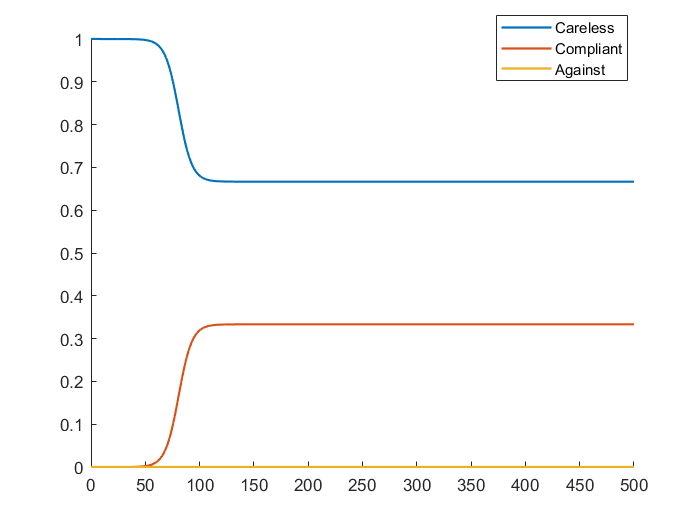
\includegraphics[width=0.7\linewidth]{1_corpo/figure/behavioural_equilibrium/r1greater1_dyn}
	\caption[Behavioural dynamic first case]{The behavioural system dynamic with $R1 > R2$ and $R1 > 1$.}
	\label{fig:r1greater1dyn}
\end{figure}
In this first scenario, as visible in figure \ref{fig:r1greater1dyn}, the Against compartment tend to zero, so the equilibrium point can be calculated as $Ca = \lambda_1/k_1$ and $Co = 1 - \lambda_1/k_1 $. 
The nullcline resulting plot is visible in \ref{fig:r1greater1nullcline}. 
\begin{figure}[h]
	\centering
	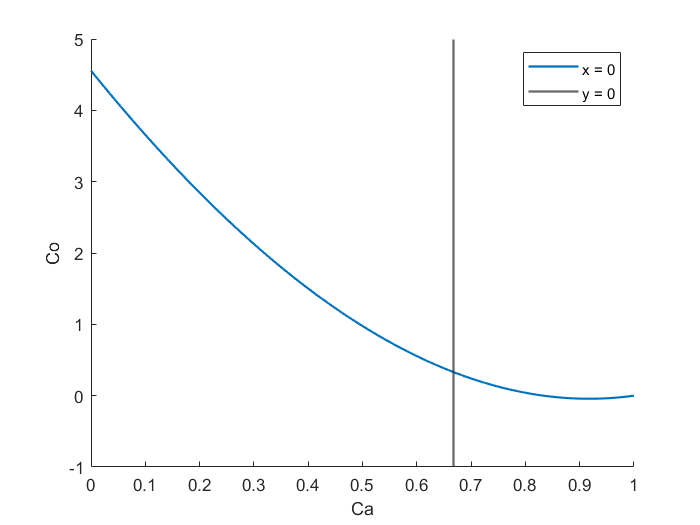
\includegraphics[width=0.7\linewidth]{1_corpo/figure/behavioural_equilibrium/r1greater1_nullcline}
	\caption[Behavioural nullcline first case]{The behavioural system nullcline lines with $R1 > R2$ and $R1 > 1$.}
	\label{fig:r1greater1nullcline}
\end{figure}

The equilibrium found as intersection of the two lines correspond to the one calculated with the numerical equation. With the Routh-Hurwitz criteria the stability of this point is verified. To evaluate if the criteria is satisfied the Jacobian matrix of the system is calculated. Then the equilibrium is used to evaluate the trace and determinant of the system in this value. To see if the equilibrium satisfies Routh-Hurwitz condition it must holds:
\begin{itemize}
	\item trace(J) $< 0$
	\item det(J) $> 0$
\end{itemize}
Both condition holds and the solution is asymptotically stable and does not depends on the initial condition.
%%%%%%%%%%%%%%%%%%

\textbf{II case:} $R_2 >1$ and $R_2> R_1$\\
The plots of the system evolution has an opposite behaviour w.r.t the first case. So here, is the Compliant compartment that tend to zero at equilibrium. 

\begin{figure}[h]
	\centering
	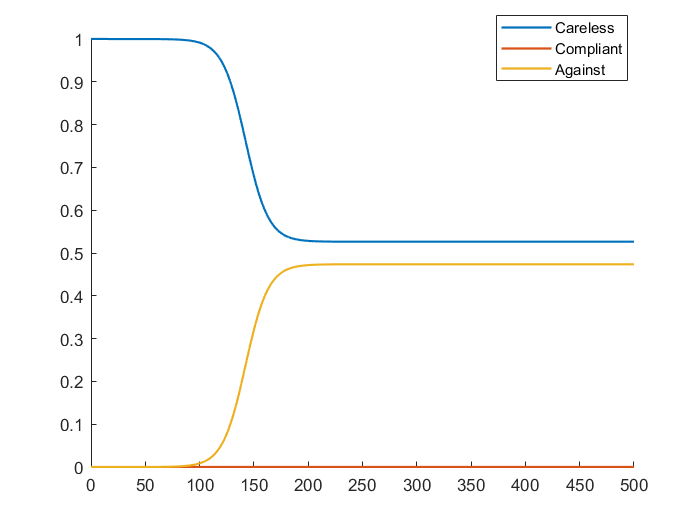
\includegraphics[width=0.7\linewidth]{1_corpo/figure/behavioural_equilibrium/r2greater1_dyn}
	\caption[Behavioural dynamic second case]{The behavioural system dynamic with $R2 > R1$ and $R2 > 1$.}
	\label{fig:r2greater1dyn}
\end{figure}
The equilibrium point can be calculated as $Ca = \lambda_2/k_2$ and $Co = 1 - \lambda_2/k_2$. 
The nullcline resulting plot is visible in \ref{fig:r2greater1nullcline}. 
\begin{figure}[h]
	\centering
	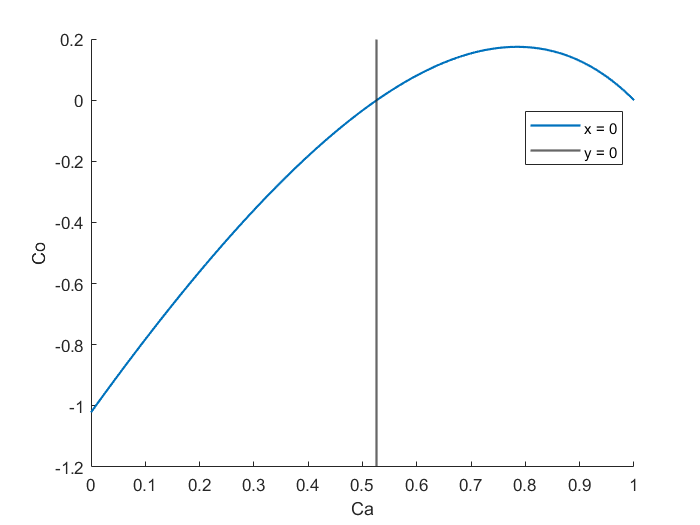
\includegraphics[width=0.7\linewidth]{1_corpo/figure/behavioural_equilibrium/r2greater1_nullcline_1}
	\caption[Behavioural nullcline second case]{The behavioural system nullcline lines with $R2 > R1$ and $R2 > 1$.}
	\label{fig:r2greater1nullcline}
\end{figure}
The equilibrium is asymptotically stable. 
%%%%%%%%%%%%%%%%%%%%%%%%%%%%

\textbf{III case:} $R_1 <1$ and $R_2<1$ \\
If both the "reproduction rates" have a value lower than one, the stable equilibrium is the one in which both Compliant and Against goes to zero. 

From the nullcline plot \ref{fig:r1r2less1nullcline}, it can be seen that there is not an intersection. The plot of the second nullcline result in a vertical line with a value grater than one. In this condition the only equilibrium is the one for which $Ca = 1$ and both $Ag$ and $Co$ are equal to zero. 
The equilibrium is asymptotically stable. 
\begin{figure}[h]
	\centering
	\subfloat[][\emph{System  evolution.}]
	{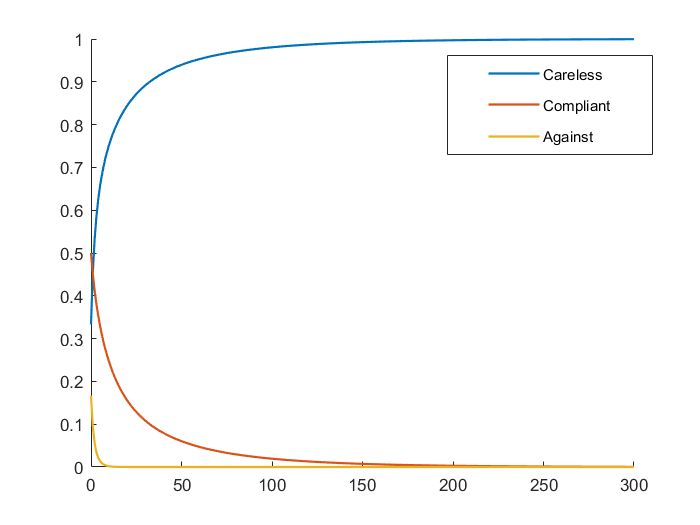
\includegraphics[width=0.47\linewidth]{1_corpo/figure/behavioural_equilibrium/r1r2less1_dyn}} \quad
	\subfloat[][\emph{Nullclines plots.}]
	{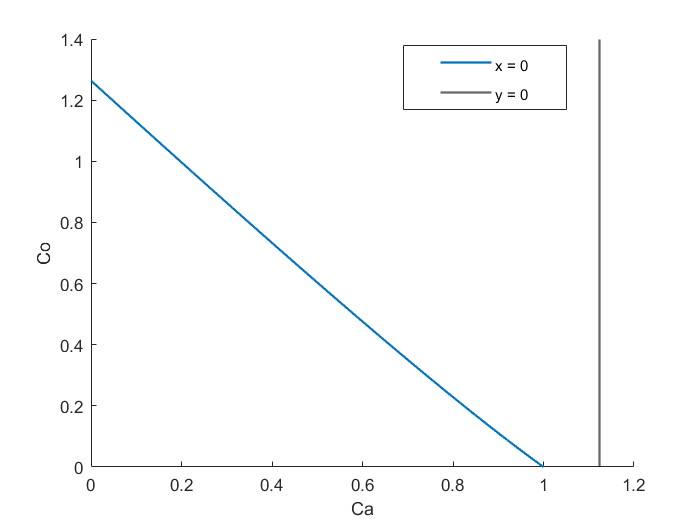
\includegraphics[width=0.47\linewidth]{1_corpo/figure/behavioural_equilibrium/r1r2less1_nullcline}} \\
	\caption[Behavioural model third case]{Behavioural system dynamics and nullcline in the case of   with $R_1 < 1$ and $R_2 < 1$.}
	\label{fig:r1r2less1dyn}
\end{figure}

%%%%%%%%%%%%%%%%%%%%%%%%%%%%

\textbf{IV case:} $R_1 = R_2$ \\
This final situation is the most difficult to analyse. In fact, due to the equal value of the two influence processes, the final equilibrium of the compartments cannot be calculated using only the previous relations, but depends also on the initial condition. 
The Careless compartment can be calculated using the same equation of previous cases, and the same value is found using both $Ca = \lambda_1/k_1$ and $Ca = \lambda_2/k_2$. As it can be seen from the system evolution and nullcline plots \ref{fig:r1r2equaldyn},at the equilibrium the Against and Compliant groups are formed by a subdivision of the $1 - Ca$ part. The initial condition have an influence on how this subdivision is composed. Using the Routh-Hurwitz criterium nothing can be said on this equilibrium because the determinant of the Jacobian have a null value.
\begin{figure}[h]
	\centering
	\subfloat[][\emph{System  evolution.}]
	{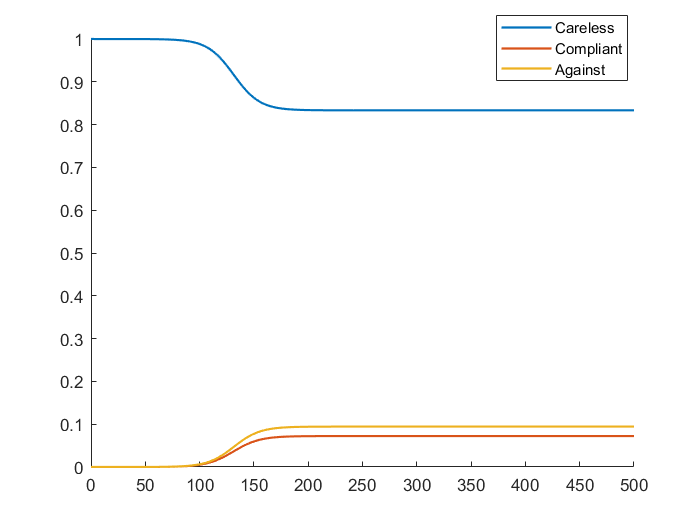
\includegraphics[width=0.47\linewidth]{1_corpo/figure/behavioural_equilibrium/r1equalr2_dyn}} \quad
	\subfloat[][\emph{Nullclines plots.}]
	{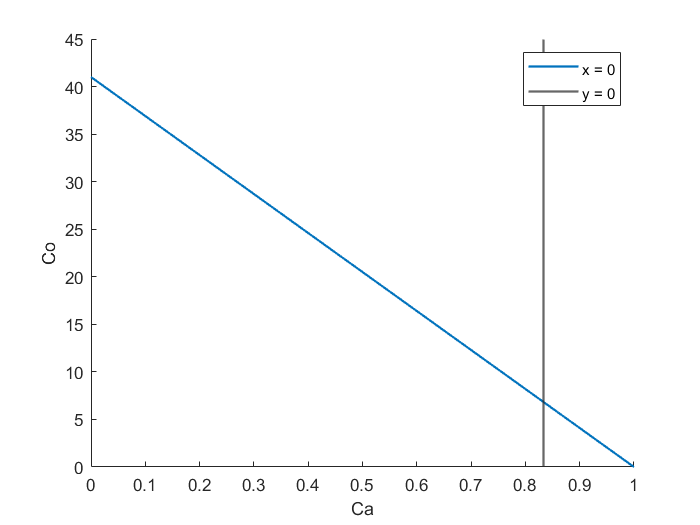
\includegraphics[width=0.47\linewidth]{1_corpo/figure/behavioural_equilibrium/r1equalr2_nullcline}} \\
	\caption[Behavioural model fourth case]{Behavioural system dynamics and nullcline in the case of   $R_1 = R_2$.}
	\label{fig:r1r2equaldyn}
\end{figure}

\subsubsection{Behavioural model experiment}
To better comprehend all the possible scenarios that can emerge with the behavioural model a simulation is performed. Four vectors are defined, one for each parameter of the model. A different simulation for each combination of the coefficient is then roll out. In this case the value of the parameters is kept constant during each simulation.
The range of variation of each parameter is the following:
\begin{itemize}
	\item $k_1$ between $0.1$ and $0.99$
	\item $k_2$ between $0.1$ and $0.99$
	\item $\lambda_1$ between $1/5$ and $1/30$ $d^{-1}$
	\item $k_1$ between $1/5$ and $1/30$ $d^{-1}$
\end{itemize}
We observe the evolution of the dynamics of all the states, and to present a summary of the effects we collect for each simulation data such as the final value of the compartment, the max peak value and the corresponding time in which the peak occur. 
Also here, for the sensitivity plots realization, the reproduction rates deriving from the combination of coefficients, equation \ref{eq:behave_rate}, are used. 

The first plots \ref{fig:subfig_sensitivity_behavioural} are heat maps about the final value reached by various compartments, varying $R_1$ and $R_2$.

\begin{figure}[h]
	\centering
	\subfloat[][\emph{Final Compliant compartment}]
	{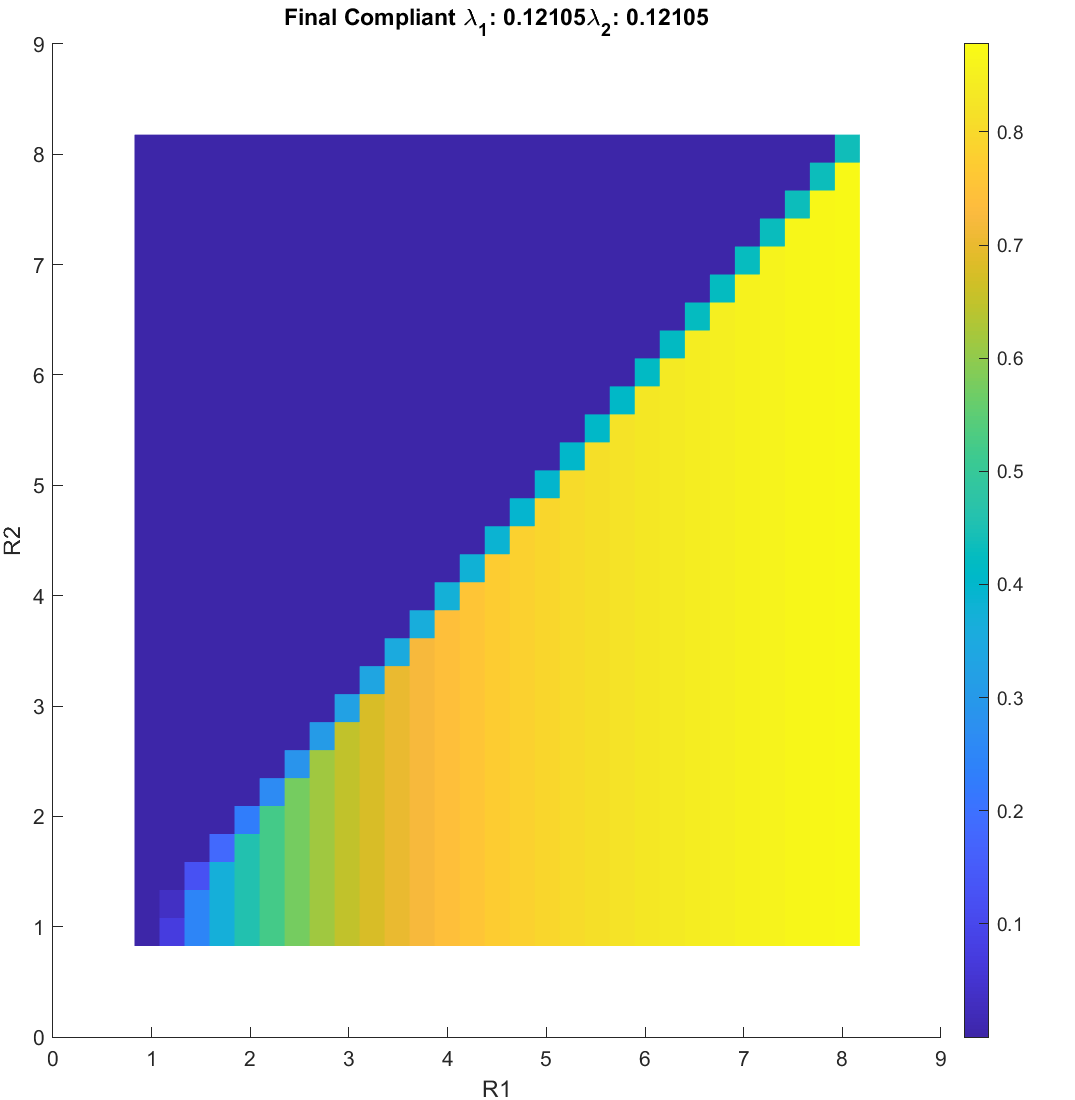
\includegraphics[width=.47\textwidth]{1_corpo/figure/behavioural_equilibrium/final_compliant_sensitivity}} \quad
	\subfloat[][\emph{Final Against compartment}]
	{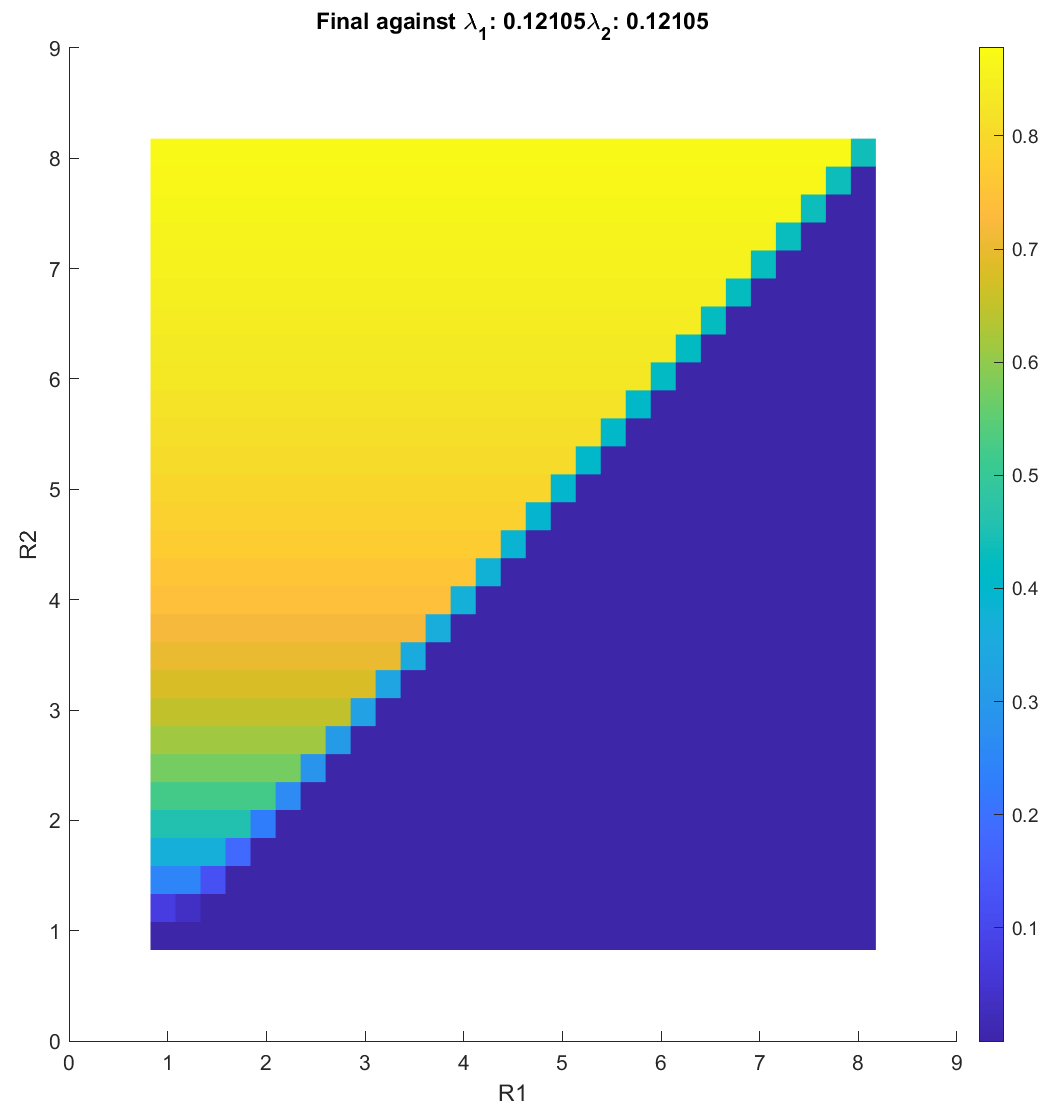
\includegraphics[width=.47\textwidth]{1_corpo/figure/behavioural_equilibrium/final_against_sensitivity}} \\
	\subfloat[][\emph{Final Careless compartment}]
	{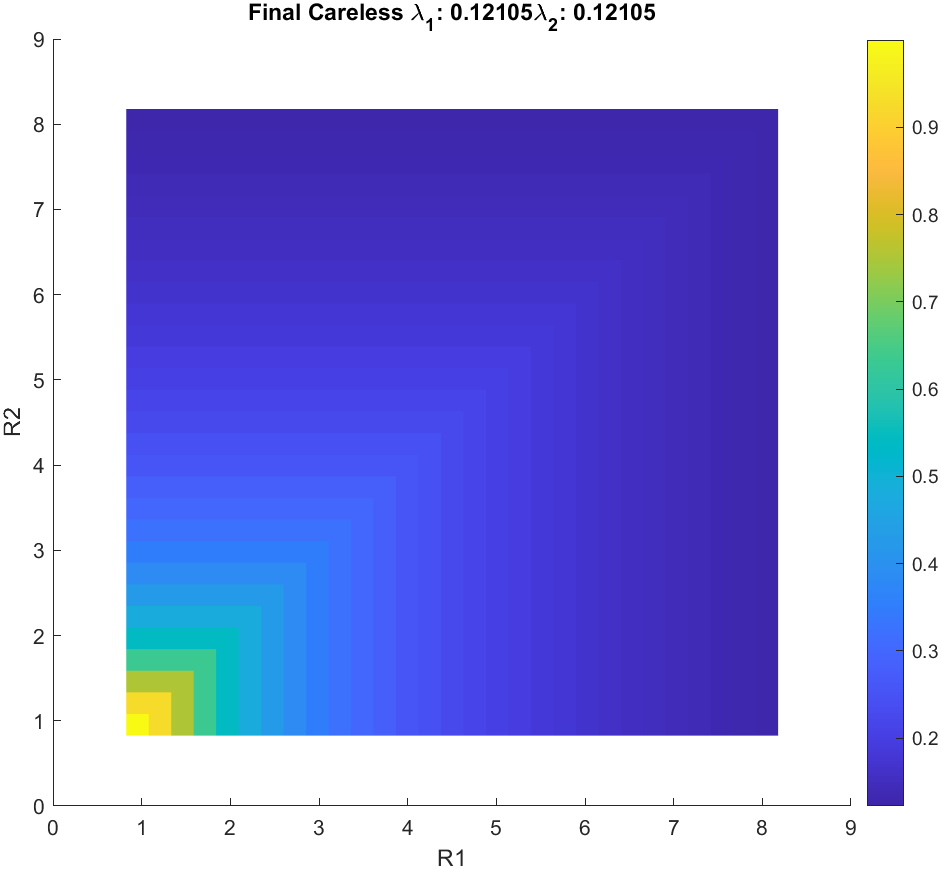
\includegraphics[width=.47\textwidth]{1_corpo/figure/behavioural_equilibrium/final_careless_sensitivity}}
	\caption[Final Behavioural compartments]{The final value reached at equilibrium by every compartment in the behavioural model.}
	\label{fig:subfig_sensitivity_behavioural}
\end{figure}

In these pictures is clearly visible the threshold effect observed in the stability analysis performed earlier. While one of the reproduction ratios becomes larger than the other, the system equilibrium is composed by the dominant group and a portion of Careless individuals.The greater is the ratio, the  smaller is the size at equilibrium of the Careless. 

Another figure in which this threshold effect can be observed is \ref{fig:subfig_sensitivity_behavioural_r1}.

\begin{figure}[h]
	\centering
	\subfloat[][\emph{Final Compliant compartment}]
	{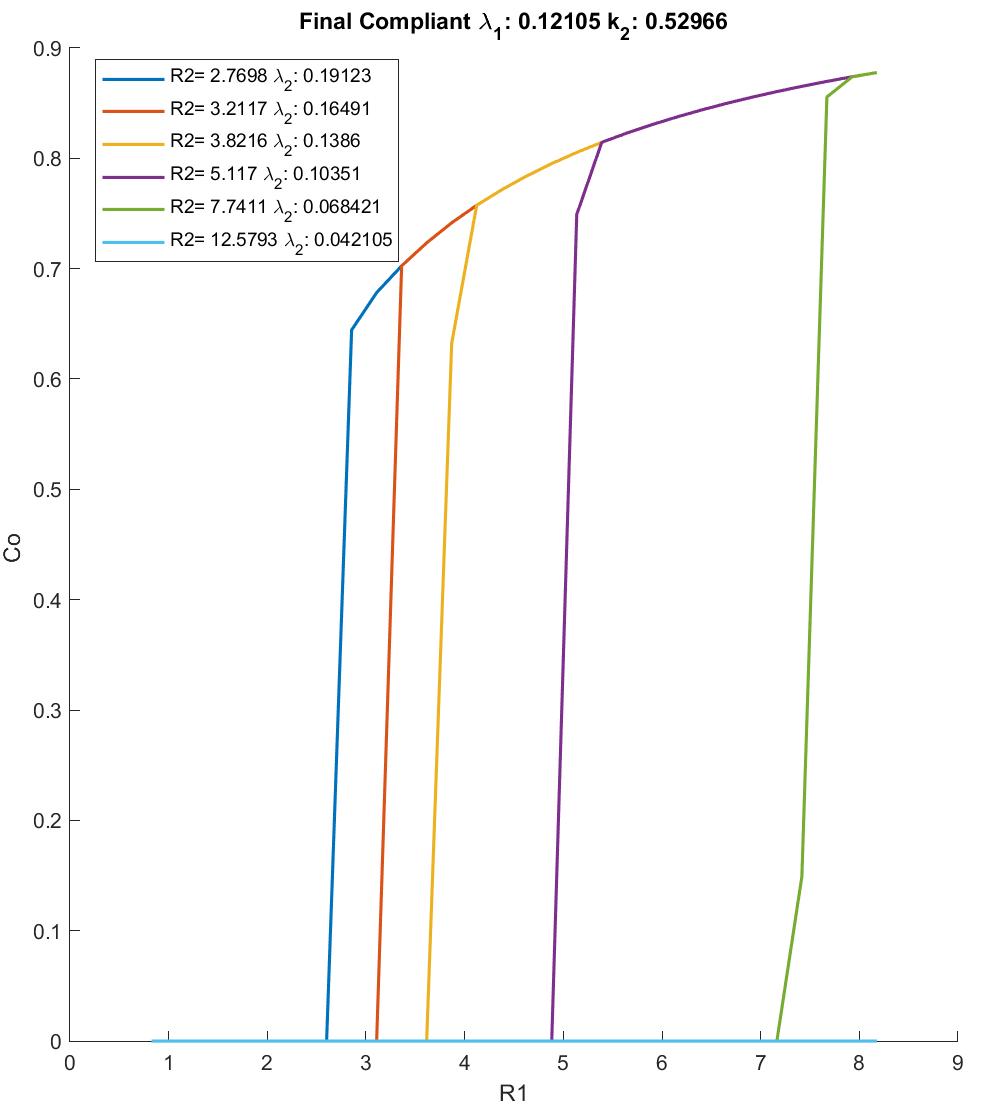
\includegraphics[height=.45\textwidth]{1_corpo/figure/behavioural_equilibrium/final_compliant_r1}} \quad
	\subfloat[][\emph{Final Against compartment}]
	{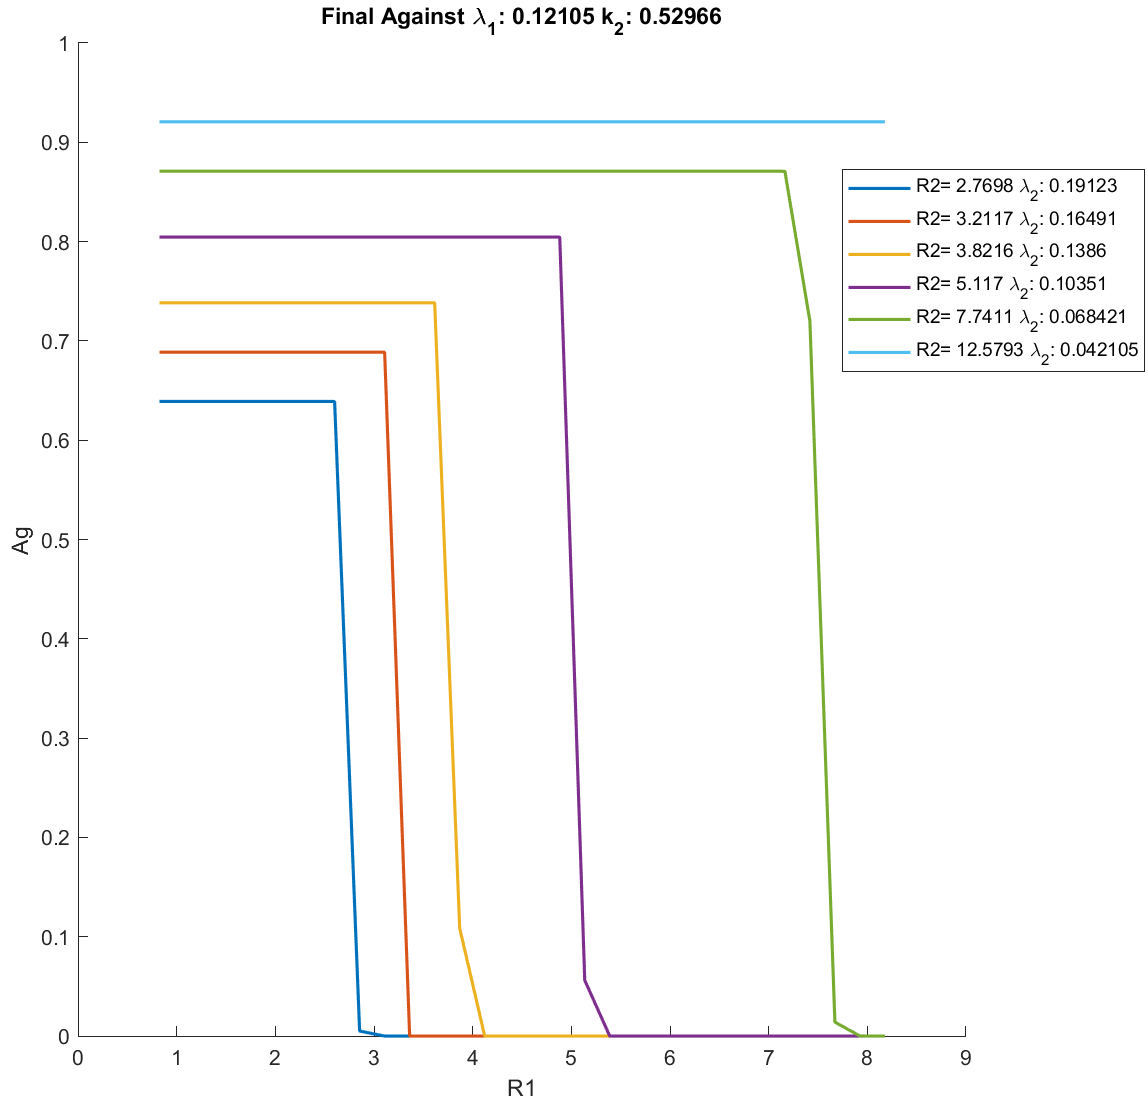
\includegraphics[height=.45\textwidth]{1_corpo/figure/behavioural_equilibrium/final_against_r1}} \\
	\subfloat[][\emph{Final Careless compartment}]
	{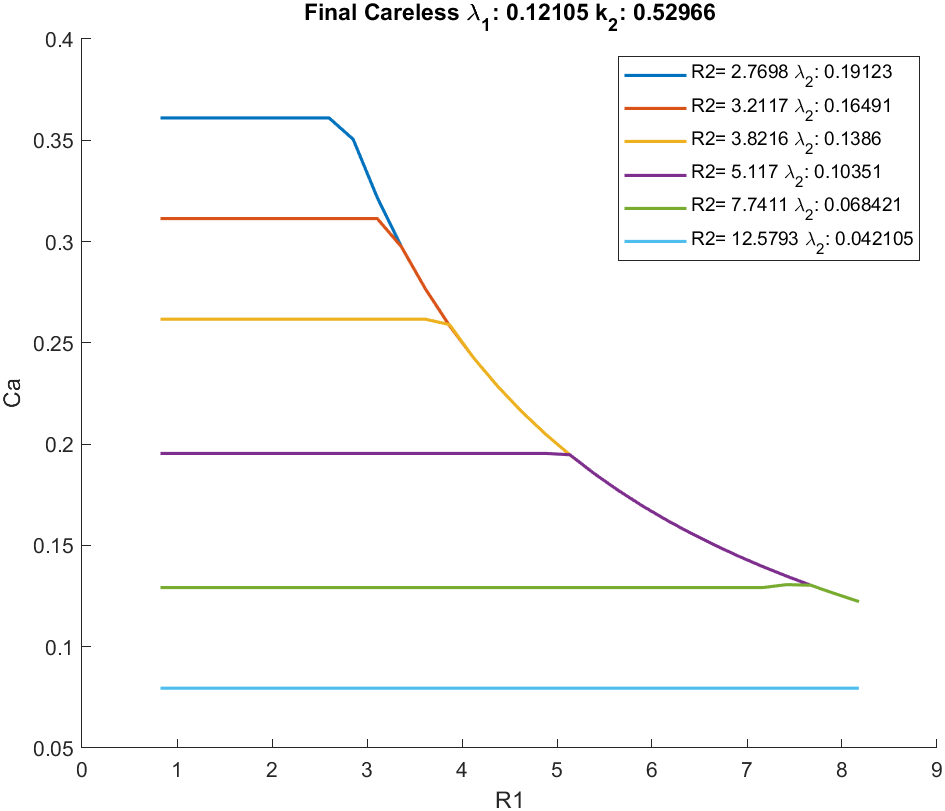
\includegraphics[height=.45\textwidth]{1_corpo/figure/behavioural_equilibrium/final_careless_r1}}
	\caption[Final Behavioural compartments varying $R_1$]{The final value reached at equilibrium by every compartment in the behavioural model varying the $R_1$ coefficient w.r.t different $R_2$ values.}
	\label{fig:subfig_sensitivity_behavioural_r1}
\end{figure}
The plots show how, for a fixed values of $\lambda_1$ and $k_2$, change the size at equilibrium of the system, varying the $k_1$ coefficient. To highlight the threshold effect due to the comparison of reproduction rates, on the x-axis is plotted the $R_1$  coefficient, that can be calculated knowing the value of  $\lambda_1$ and $k_1$. For the same reason, different $R_2$ situations are represented. 

The threshold effect is clearly visible also here. Looking at the Compliant and Against final values it can also be seen that after the $R_1$ reproductive coefficient is became dominant, the  increase is the final size observed in the Compliant plot is due to the decrease in the Careless compartment. 

%Provo a scrivere, ma si va tutto molto bene
%L'inglese, come disse Daniele è da sistemare, però sono su una buona strada...




\chapter{Models description and analysis}
\section{Behavioral epidemic model}

The model is composed of two layer coupled together. A disease one describing the evolution of an epidemic and a behaviour one in which there are different behaviour during the epidemic development.
The behavioral layer has three possible compartments: 

\begin{itemize}
	\item Heedless, people careless of the risk associated to the infection;
	\item Compliant, composed by person that want avoid to become infected or infect others
	\item Against, who not consider a new infection developing as a risk for its safety and not use protection or change its behaviour during the epidemic. 
\end{itemize}
The symbols used to represent these compartments are $H$, $C$, $A$.
This behaviour structure is coupled with a SIRS epidemic model.

The resulting system is described by the following set of differential equations \ref{eq:epi_behavioural_eq}: 
\begin{equation}
	\begin{cases}
		\dot{SH} = - \phi k_1 SH \cdot C - k_2 SH \cdot A + \lambda_1 SC + \lambda_2 SA + \delta(1-\phi_n)RC - \beta SH \cdot I\\
		\dot{SC} = \phi k_1 SH \cdot C + \delta \phi_n RC - \lambda_1 SC - \beta \rho SC \cdot I  \\
		\dot{SA} = k_2 SH \cdot A - \lambda_2 SA - \beta SA \cdot I + \delta RA \\
		\dot{IC} = \beta \rho SC \cdot I + \beta SH \cdot I + \phi k_3 IA \cdot C - \lambda_3 IC -  k_4 IC \cdot A + \lambda_4 IA - \gamma IC\\
		 \dot{IA} = \beta SA \cdot I - \phi k_3 IA \cdot C + \lambda_3 IC + k_4 IC \cdot A - \lambda_4 IA - \gamma IA\\
		 \dot{RC} = \gamma IC - k_6 RC \cdot A + \lambda_6 RA + \phi k_5 RA \cdot C - \lambda_5 RC - \delta RC\\
		 \dot{RA} = \gamma IA + k_6 RC \cdot A - \lambda_6 RA - \phi k_5 RA \cdot C + \lambda_5 RC - \delta RA\\
	\end{cases}
	\label{eq:epi_behavioural_eq}
\end{equation}

Some specifications:
\begin{itemize}
	\item $A = SA + IA + RA$ the totality of Against group.
	\item $C = SC + IC + RC$ the totality of Compliant group.
	\item $I = \epsilon \cdot IC + IA$ the part of infected people participating into the infection process.
	\item $\phi$ is awareness a parameter that account for the current state of epidemic and influence the behaviour persuasion between groups. It can be modelled in different ways. 
	\item $\phi_n$ it is the awareness normalized, used to split the population while re entering in the susceptible class in the Heedless or Compliant group. 
	\item $\rho$ is the protection factor that Compliant people have and reduce their possibility of become infected.
	\item $\beta$ is the infectivity rate associated with the disease.
	\item $\gamma$ is the rate of infection duration.
	\item $\delta$ is the recovery rate from the state $R$ to return in the $S$ one. 
	\item $\epsilon$ specify the part of compliant infected that participate to the infection process.
\end{itemize}


\subsection{Basic reproduction number calculation}
The first analysis that can be performed on the behavioral disease model is to estimate its basic reproduction number. It is defined as the spectral radius of the next-generation matrix. Using the method outlined in \cite{arino2007} and now briefly described this quantity is calculated. 
Consider a simple disease model in which $x \in R^n$ represents the set of infected compartments, $y \in R^n$ the set of susceptibles compartments, and $z \in R^k$ the set of compartments removed to the infection due to recovery. 

To describe the evolution of the system the following notation using matrices is adopted: 
\begin{itemize}
	\item D is a $m \times m$ diagonal matrix; the diagonal elements are the relative susceptibilities of the corresponding susceptible class.
	\item $\Pi$ is a $n \times m$ matrix in which the $(i,j)$ element is the fraction of susceptible in the $j^{th}$ compartment that goes into the $i^{th}$ infective compartment.
	\item $b$ is an n-dimensional row vector of relative
	horizontal transmissions.
	\item $\beta$ multiplies the $b$ vector and is a scalar factor representing infectivity. It can be constant or a function of other parameters, such as incidence for example. 
	
	\item $V$ is a $n \times n$ matrix describing the transition between the infected state through death and recovery. 
	\item $g(s, i,r)$ is a continuous function representing the inlet of uninfected through birth or immigration. 
	\item $h(s, i, r)$ is also a function but used for the flow into and out of the recovered compartment because of natural immunity or vaccination.
\end{itemize} 

The resulting disease model is represented by the system:

\begin{equation}
	\begin{cases}
		s' = g(s,i,r) - D s \beta(s,i,r) b i\\
		i' = \Pi D s \beta(s,i,r) b i - V i\\
		r' = h(s,i,r) + W i \\		
	\end{cases}
	\label{eq:epi_ro_eq}
\end{equation}

Using the defined matrices, according to \cite{arino2007} the basic reproduction number $R_0$ for the model \ref{eq:epi_ro_eq} at a disease free equilibrium $(s_0, 0, r_0)$ is given by:
\begin{equation}
R_0 = \beta b V^{-1} \Pi D s_0
\label{eq:R_0_eqn}
\end{equation}

The disease-free equilibrium is defined as a locally stable equilibrium of the system in which there is no disease and in the sense that a solution starting close to $(s_0, 0, r_0)$ remains close to this state. 

Considering the system dynamic presented in \ref{eq:epi_behavioural_eq}, it can be rewritten in the matrix form expressed in  \ref{eq:epi_ro_eq} as: 

\begin{align*}
\Pi & = 
\begin{bmatrix}
	\rho & 1 & 0 \\
	0 & 0 & 1
\end{bmatrix} &
D & = 
\begin{bmatrix}
	1 & 0 & 0 \\
	0 & 1 & 0\\
	0 & 0 & 1
\end{bmatrix} & 
s & = 
\begin{bmatrix}
	SC \\
	SH\\
	SA 
\end{bmatrix} \\
\\
b & = \begin{bmatrix}
	\epsilon & 1
\end{bmatrix} & 
V & = 
\begin{bmatrix}
	k_4 A + \lambda_3 + \gamma & - \phi k_3  C - \lambda_4\\
	- k_4 A - \lambda_3 & \phi k_3 C + \gamma + \lambda_4
\end{bmatrix} & 
i & = 
\begin{bmatrix}
	IC \\
	IA
\end{bmatrix}
\\
\end{align*}


The resulting $R_0$ find with this method is: 
\begin{figure}
	\centering
	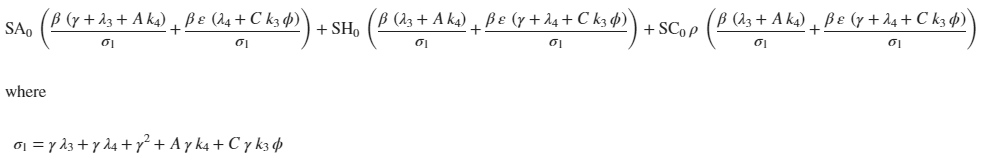
\includegraphics[width=0.99\linewidth]{1_corpo/figure/r0/ro_epidemic_behavioural}
	\caption[reproduction number of epidemic behaviour model.]{Basic reproduction number of the epidemic behaviour model.}
	\label{fig:roepidemicbehavioural}
\end{figure}



\subsubsection{$I$ case: $R_0$ first evaluation}

A first evaluation of the $R_0$ is done using equation \ref{eq:R_0_eqn} and assuming that at the beginning of an epidemic, the majority of the population is in the $SH$ compartment, while SC, SA, and also the A and C groups are close to zero. 
An initial tentative calculation for the value is done using a set of values assigned to the rest of the coefficients in the matrices.
For reference, the following values are used:

\begin{align*}
\beta &= 0.40  &\gamma &= 0.35 & \rho &= 0.65 &  \epsilon &= 0.15 \\
k_3 &= 0.49 & k_4 &= 0.243 & \lambda_3 &= 0.143 & \lambda_4 &= 0.143 \\
SC_0 & = 50/60e6 & SA_0 &= 50/60e6 & C &= A = SC_0 & SH_0 & = 1 - SC_0- SA_0\\ 	
\end{align*}


With these coefficient values, considering separately the epidemic and behavioral layers the basic reproduction values are:
 \begin{align*}
 	R_0^{SIR} &= \frac{\beta}{\gamma} = 1.1429 \\
 	R_3^{behav} & = \frac{k_3}{\lambda_3} =  3.3566  \\
 	R_4^{behav} & = \frac{k_4}{\lambda_4} = 1.6993 \\
 \end{align*}
   
In this situation, an epidemic can spread, in fact $R_0^{SIR} >1$, and looking at the behavior of people the complaints, associated with $R_3^{behav}$, have a larger influence than the one of the "against" group.

The epidemic-behaviour reproduction number found using the formula and assuming an initial awareness equal to $0.5$ is 
\[R_0^{epi-behav} = 0.3898\]

It is immediately noticed that the reproduction number is way below the threshold value of 1. According to the theorem presented in \cite{arino2007} there cannot be the spread of disease if the initial $R_0$ is under this value. A simulation of the system dynamic confirms this situation. Observing figure \ref{fig:infected00_epi_behav} can be seen that the number of infected tends to decrease and goes to zero. Then the majority of the population remains in the Susceptible compartment, splitting into compliant and heedless subgroups. This is due to the strongest attractivity of compliant behavior simulated in this scenario.  

\begin{figure}[h]
	\centering
	\subfloat[][\emph{susceptibles compartments}]
	{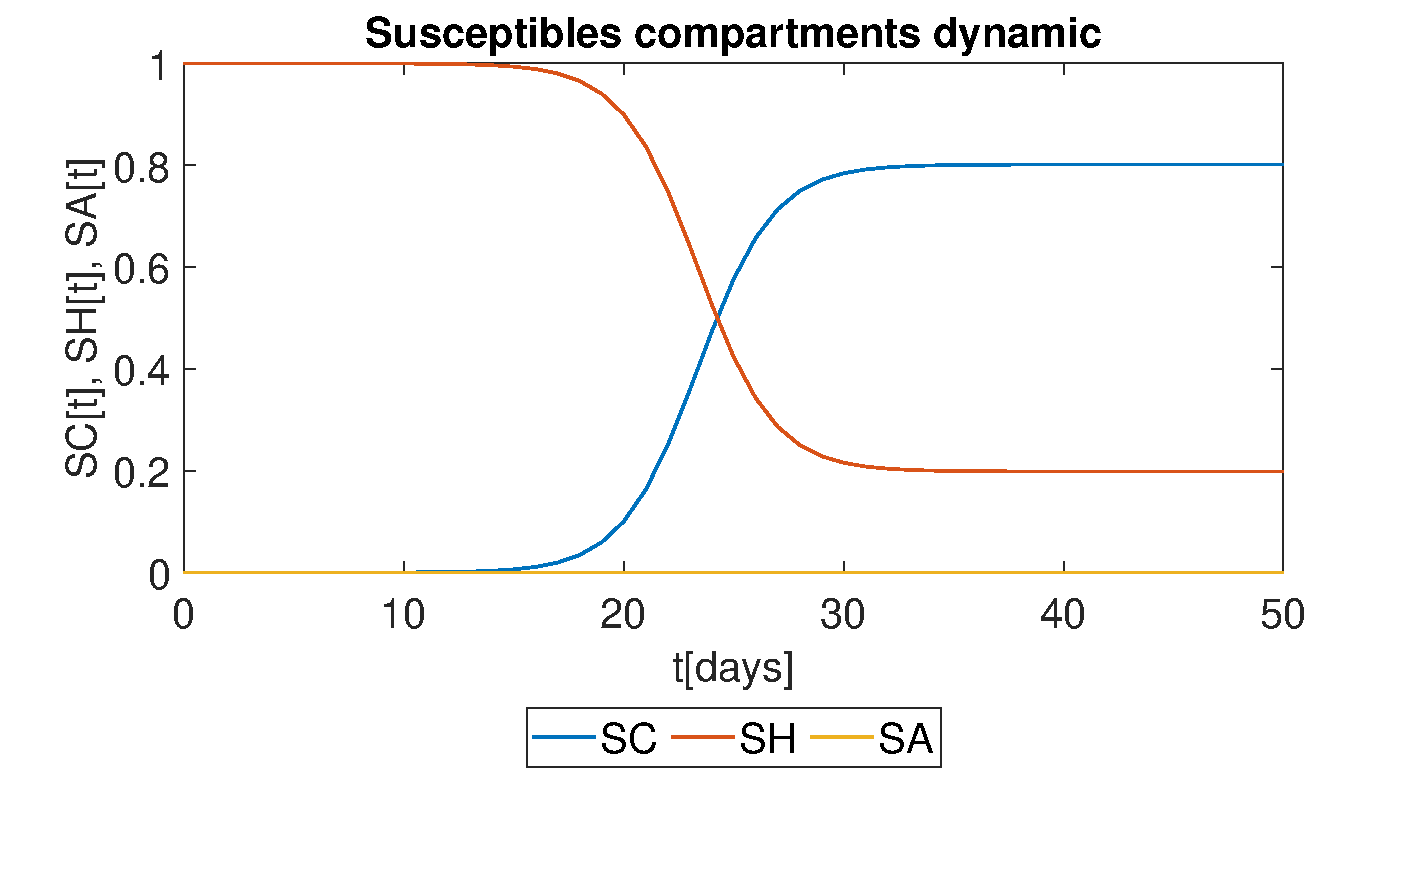
\includegraphics[width=.45\textwidth]{1_corpo/figure/r0/susceptible00_epi_behav}} \quad
	\subfloat[][\emph{infected compartments}]
	{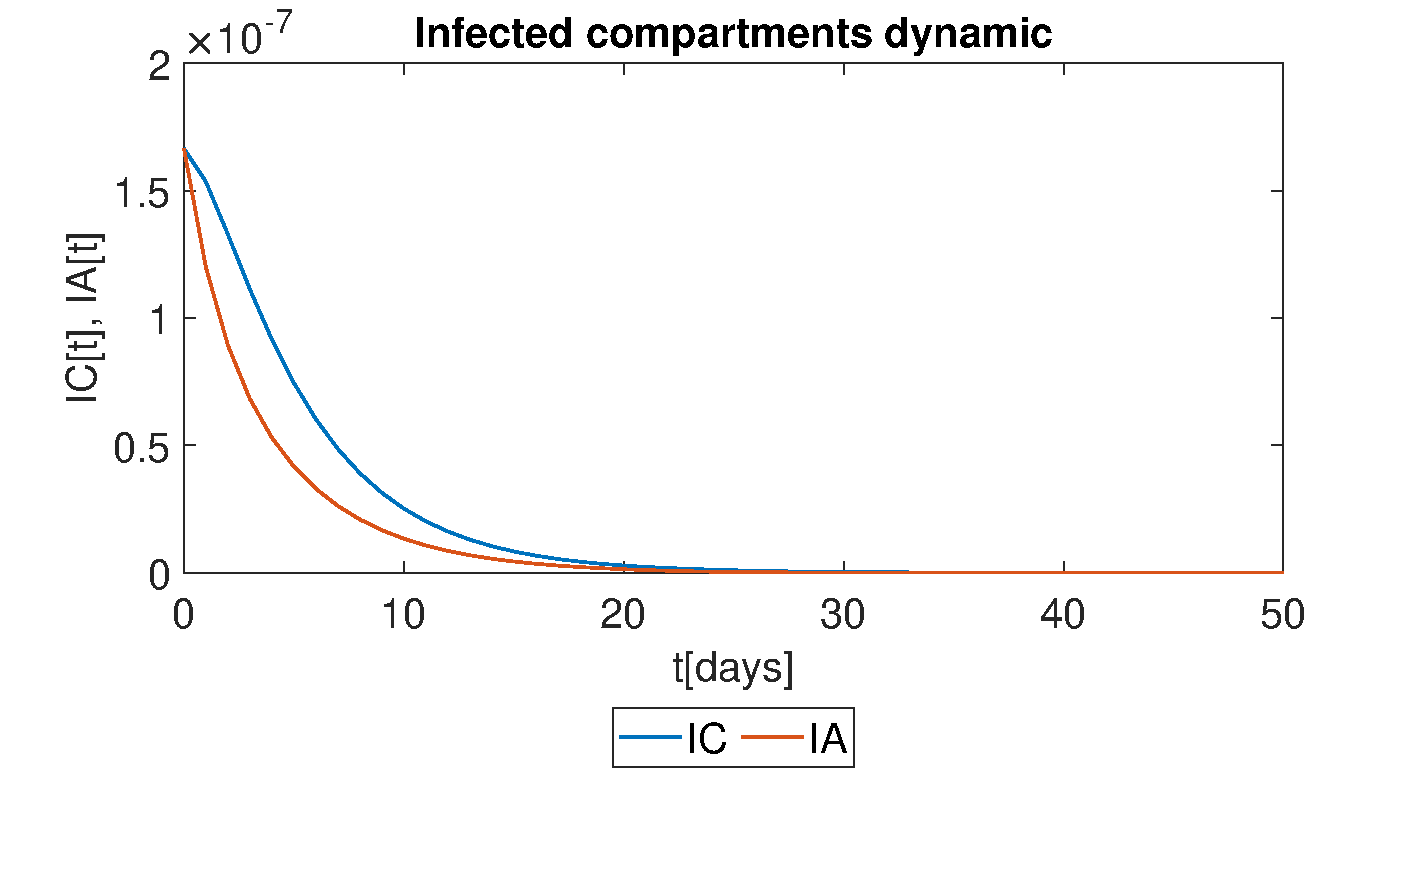
\includegraphics[width=.45\textwidth]{1_corpo/figure/r0/infected00_epi_behav}} \\
	\subfloat[][\emph{recovered compartment}]
	{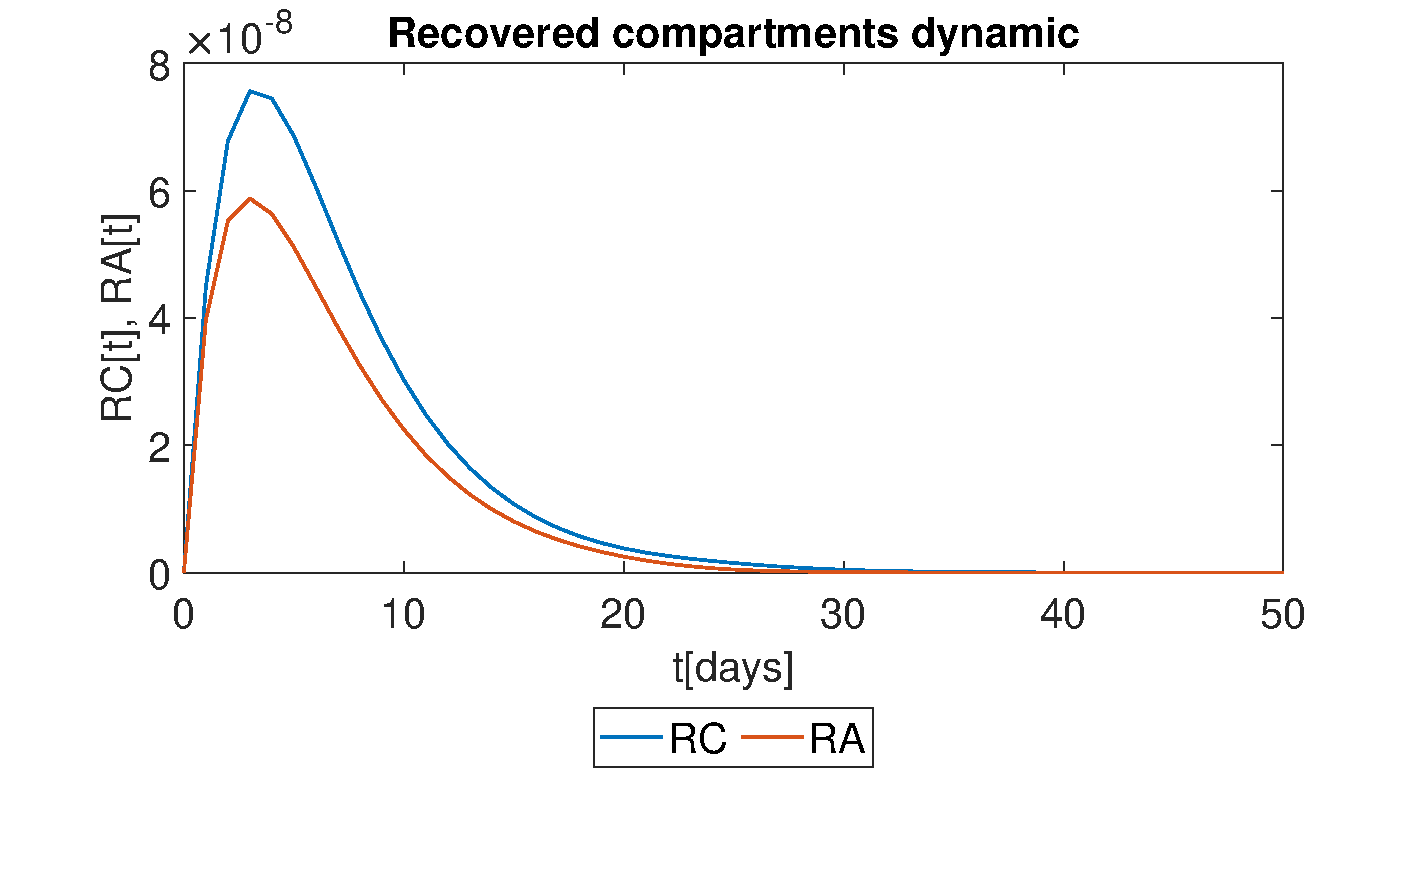
\includegraphics[width=.45\textwidth]{1_corpo/figure/r0/recovered00_epi_behav}}
	\caption[Epidemic behavioral model $R_0$]{Evolution of the behavioral epidemic model, with fixed parameters for the coefficients and an initial reproduction rate less than $1$. It is observed that there aren't conditions for an epidemic to spread.}
	\label{fig:infected00_epi_behav}
\end{figure}

\subsubsection{$II$ case: how parameters influence the $R_0$ value}

A second test performed on the find $R_0^{epi-behav}$ wants to understand what are the parameters that influence more its value. The aim is to find which combination of coefficients can have a critical impact in the first phase of the disease and cause an overshoot of the threshold value. The value of the reproductive rate is then calculated varying the coefficients and the results are now presented in \ref{fig:r0_epi_behav_coef}. 

\begin{figure}[h]
	\centering
	\subfloat[][\emph{$R_0$ varying the initial population value in susceptible compliant and susceptible against group. The more the population is against the higher the reproductive ratio.}]
	{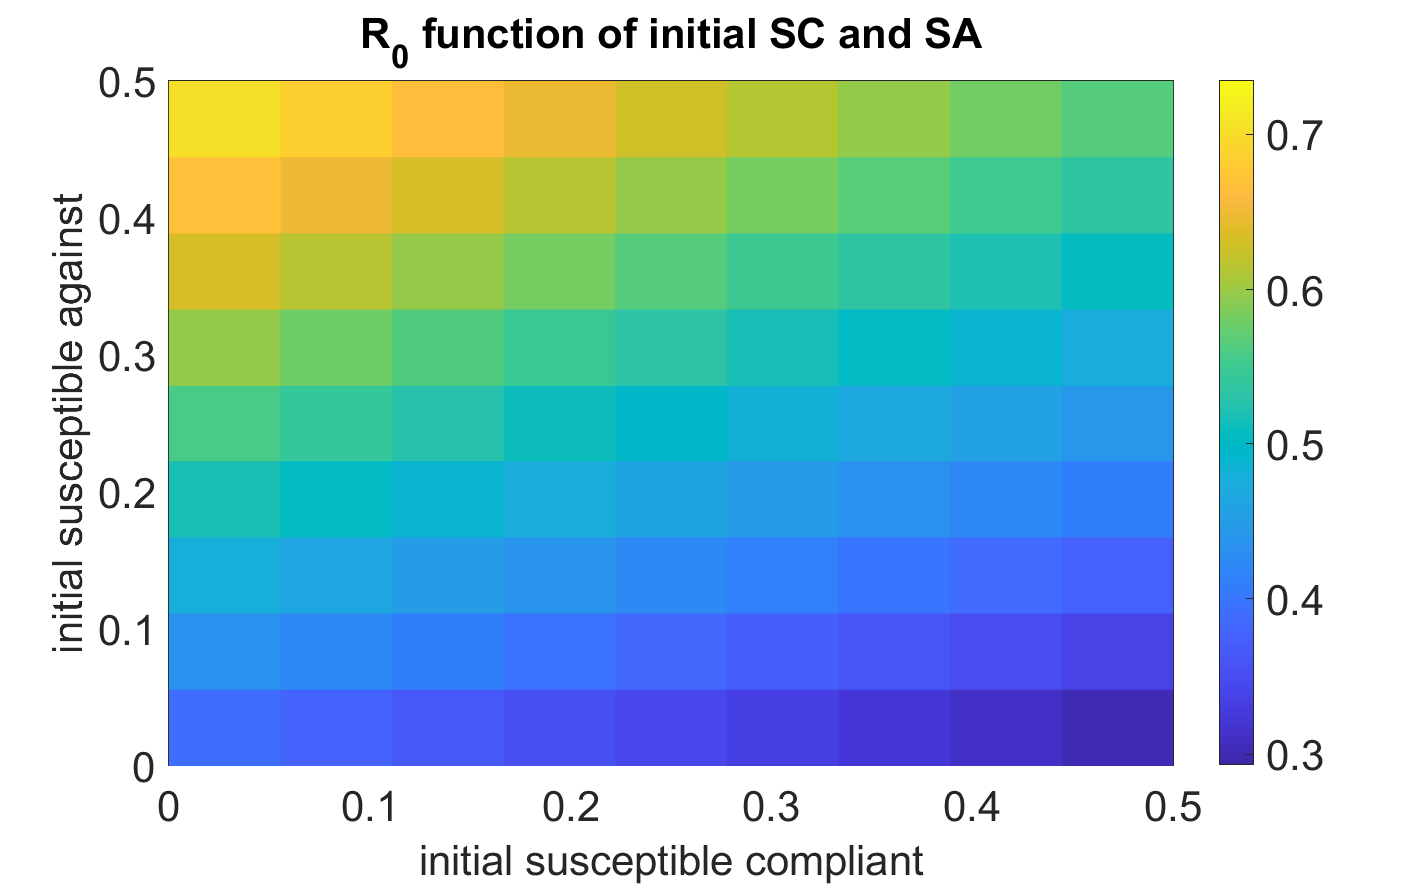
\includegraphics[width=.45\textwidth]{1_corpo/figure/r0/r0_epi_behav_SC_SA}} \quad
	\subfloat[][\emph{$R_0$ varying the number of initial compliant susceptible and the parameter ruling the efficacy of adopting a safe behavior and avoiding contracting the disease. The lower is $\rho$ the higher is the probability of not becoming infected.}]
	{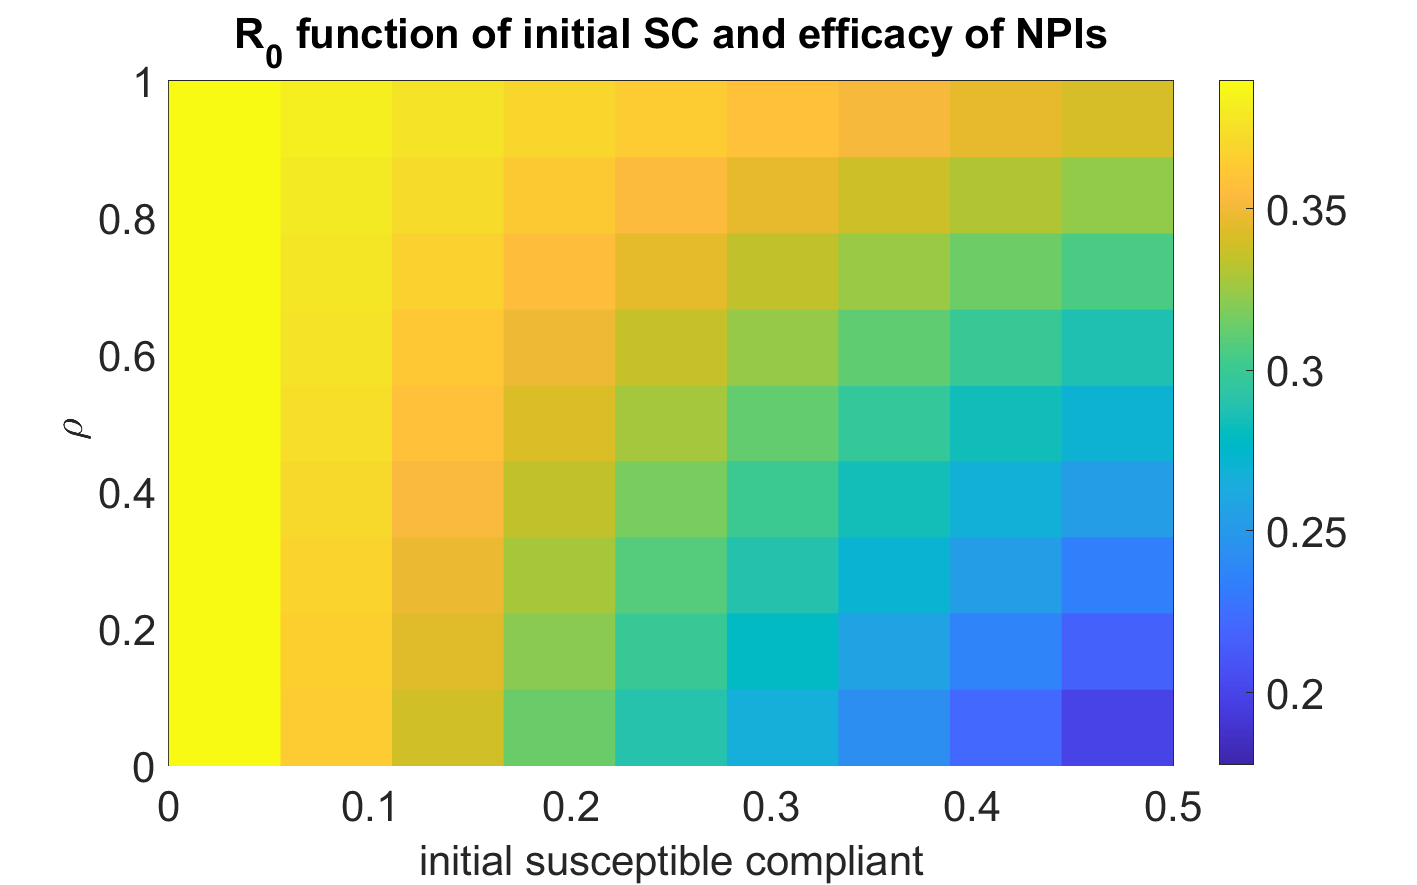
\includegraphics[width=.45\textwidth]{1_corpo/figure/r0/r0_epi_behav_SC_rho}} \\
	\subfloat[][\emph{The influence of the awareness parameter on the $R_0$.}]
	{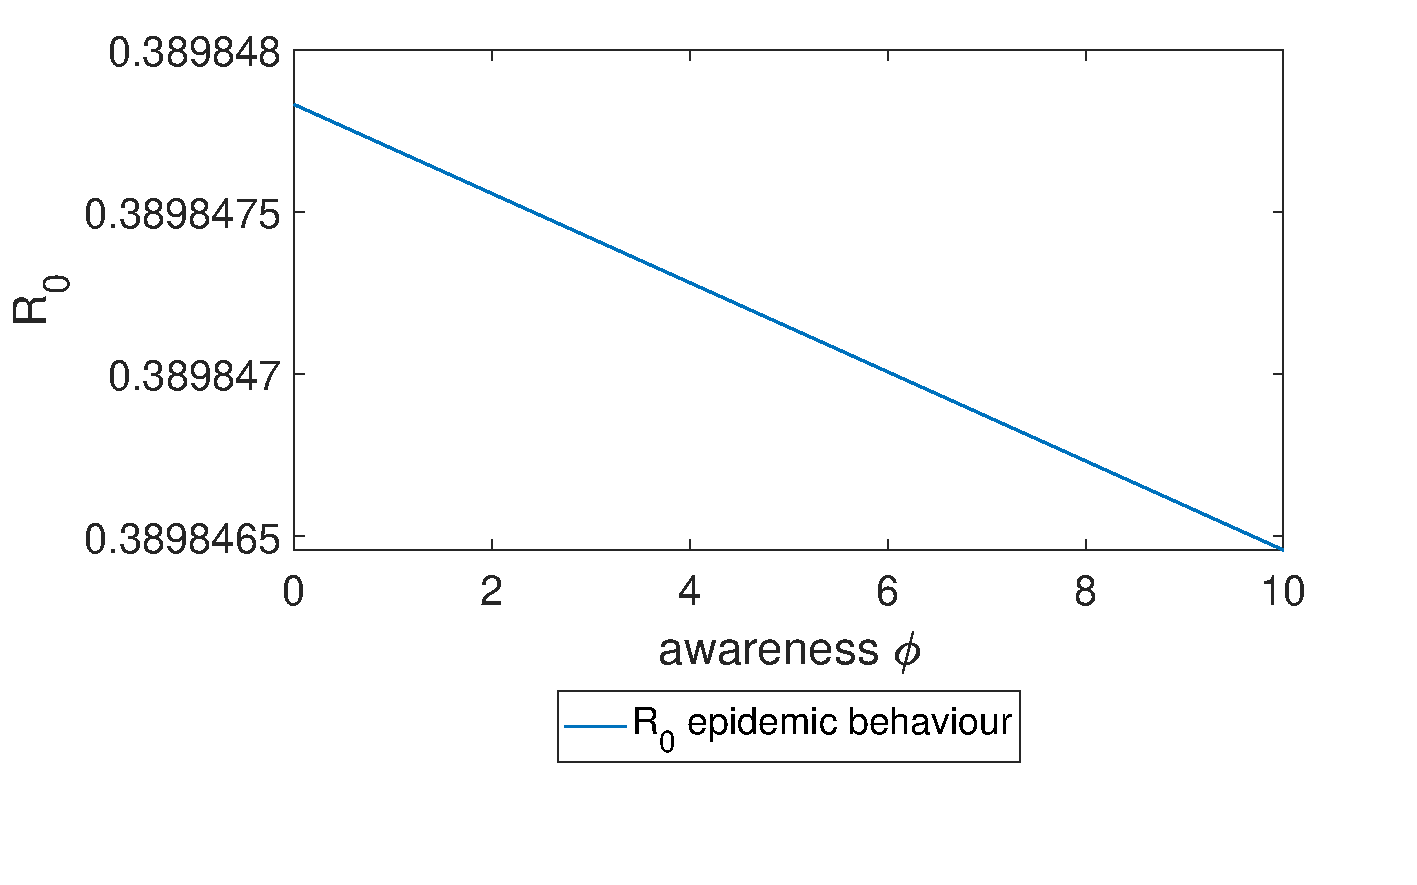
\includegraphics[width=.45\textwidth]{1_corpo/figure/r0/r0_epi_behav}}
	\caption[Epidemic behavioral $R_0$ coefficients ]{Value of $R_0^{epi-behav}$ varying some parameters and maintaining constant all the other initial conditions.}
	\label{fig:r0_epi_behav_coef}
\end{figure}


The case shown in figure \ref{fig:r0_epi_behav_coef} is an example of how changes the reproductive rate value. The most interesting observation is that the value of awareness practically does not modify the $R_0$. Instead, it can be observed a threshold in the number of initial susceptible compliant for which the reproductive rate becomes smaller, depending on the efficacy of the protective behavior. If there are less than $5\%$ of the population in the compliant group, for any value of $\rho$ the reproductive rate does not change. 